\documentclass[aspectratio=169]{../latex_main/tntbeamer}  % you can pass all options of the beamer class, e.g., 'handout' or 'aspectratio=43'
\usepackage{dsfont}
\usepackage{bm}
\usepackage[english]{babel}
\usepackage[T1]{fontenc}
%\usepackage[utf8]{inputenc}
\usepackage{graphicx}
\graphicspath{ {./figures/} }
\usepackage{algorithm}
\usepackage[ruled,vlined,algo2e,linesnumbered]{algorithm2e}
\usepackage{hyperref}
\usepackage{booktabs}
\usepackage{mathtools}

\usepackage{amsmath,amssymb}

\DeclareMathOperator*{\argmax}{arg\,max}
\DeclareMathOperator*{\argmin}{arg\,min}

\usepackage{amsbsy}
\newcommand{\vect}[1]{\bm{#1}}
%\newcommand{\vect}[1]{\boldsymbol{#1}}

\usepackage{pgfplots}
\pgfplotsset{compat=1.16}
\usepackage{tikz}
\usetikzlibrary{trees} 
\usetikzlibrary{shapes.geometric}
\usetikzlibrary{positioning,shapes,shadows,arrows,calc,mindmap}
\usetikzlibrary{positioning,fadings,through}
\usetikzlibrary{decorations.pathreplacing}
\usetikzlibrary{intersections}
\pgfdeclarelayer{background}
\pgfdeclarelayer{foreground}
\pgfsetlayers{background,main,foreground}
\tikzstyle{activity}=[rectangle, draw=black, rounded corners, text centered, text width=8em]
\tikzstyle{data}=[rectangle, draw=black, text centered, text width=8em]
\tikzstyle{myarrow}=[->, thick, draw=black]

% Define the layers to draw the diagram
\pgfdeclarelayer{background}
\pgfdeclarelayer{foreground}
\pgfsetlayers{background,main,foreground}

% Requires XeLaTeX or LuaLaTeX
%\usepackage{unicode-math}

\usepackage{fontspec}
%\setsansfont{Arial}
\setsansfont{RotisSansSerifStd}[ 
Path=../latex_main/fonts/,
Extension = .otf,
UprightFont = *-Regular,  % or *-Light
BoldFont = *-ExtraBold,  % or *-Bold
ItalicFont = *-Italic
]
\setmonofont{Cascadia Mono}[
Scale=0.8
]

% scale factor adapted; mathrm font added (Benjamin Spitschan @TNT, 2021-06-01)
%\setmathfont[Scale=1.05]{Libertinus Math}
%\setmathrm[Scale=1.05]{Libertinus Math}

% other available math fonts are (not exhaustive)
% Latin Modern Math
% XITS Math
% Libertinus Math
% Asana Math
% Fira Math
% TeX Gyre Pagella Math
% TeX Gyre Bonum Math
% TeX Gyre Schola Math
% TeX Gyre Termes Math

% Literature References
\newcommand{\lit}[2]{\href{#2}{\footnotesize\color{black!60}[#1]}}

%%% Beamer Customization
%----------------------------------------------------------------------
% (Don't) Show sections in frame header. Options: 'sections', 'sections light', empty
\setbeamertemplate{headline}{empty}

% Add header logo for normal frames
\setheaderimage{
	% 
\includegraphics[height=\logoheight]{figures/TNT_darkv4.pdf}
	
\includegraphics[height=\logoheight]{../latex_main/figures/luh_logo_rgb_0_80_155.pdf}
	% 
\includegraphics[height=\logoheight]{figures/logo_tntluh.pdf}
}

% Header logo for title page
\settitleheaderimage{
	% 
\includegraphics[height=\logoheight]{figures/TNT_darkv4.pdf}
	
\includegraphics[height=\logoheight]{../latex_main/figures/luh_logo_rgb_0_80_155.pdf}
	% 
\includegraphics[height=\logoheight]{figures/logo_tntluh.pdf}
}

% Title page: tntdefault 
\setbeamertemplate{title page}[tntdefault]  % or luhstyle
% Add optional title image here
%\addtitlepageimagedefault{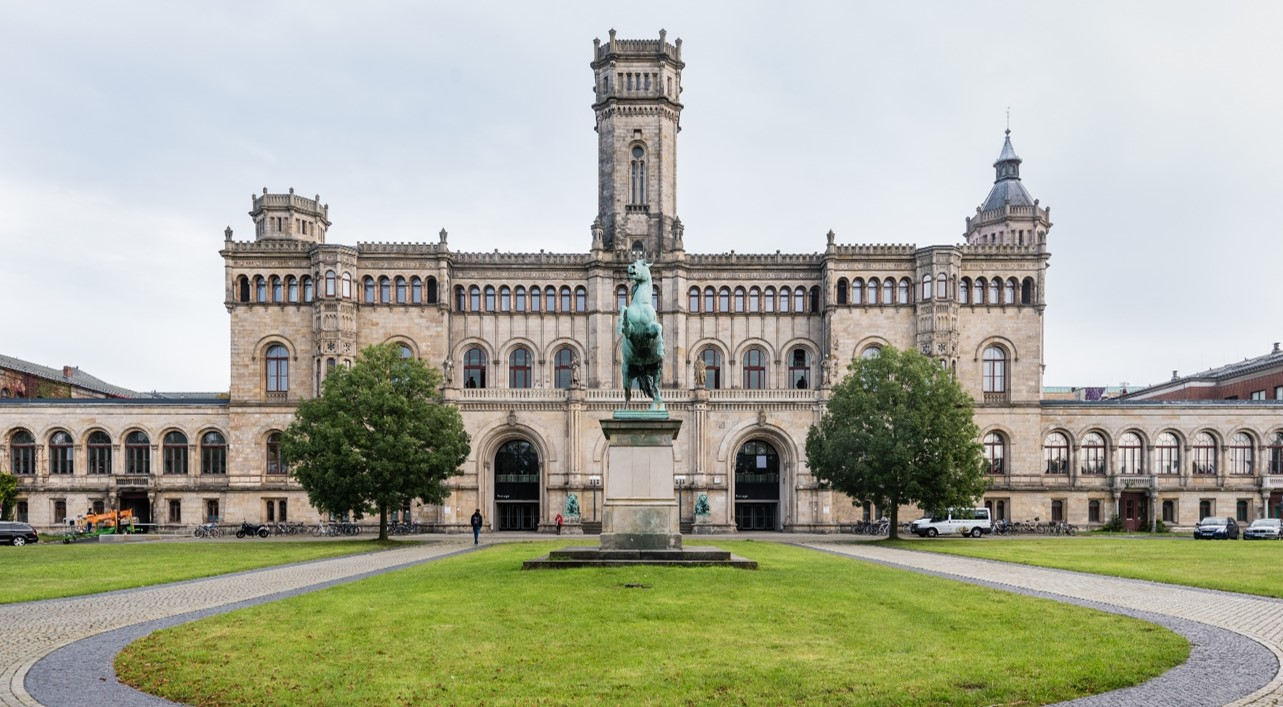
\includegraphics[width=0.65\textwidth]{figures/luh_default_presentation_title_image.jpg}}

% Title page: luhstyle
% \setbeamertemplate{title page}[luhstyle]
% % Add optional title image here
% \addtitlepageimage{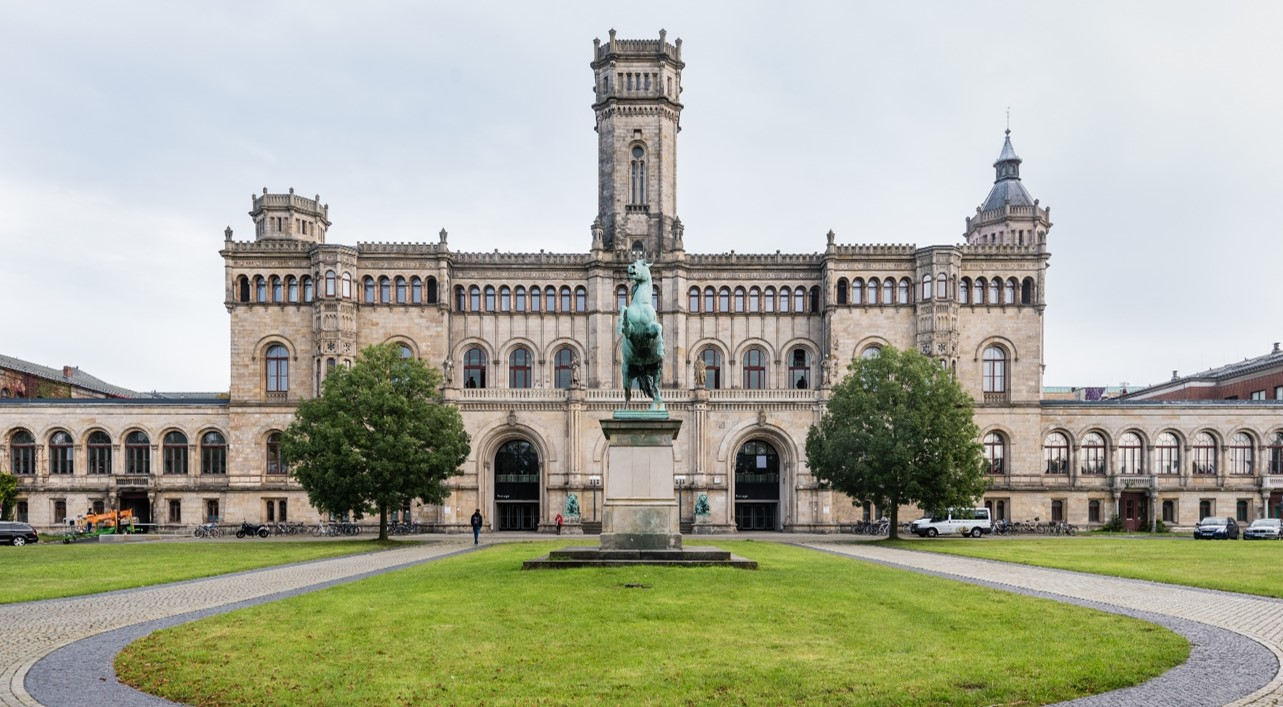
\includegraphics[width=0.75\textwidth]{figures/luh_default_presentation_title_image.jpg}}

\author[Abedjan \& Lindauer]{Ziawasch Abedjan \& Marius Lindauer\\[1em]
	
\includegraphics[height=\logoheight]{../latex_main/figures/luh_logo_rgb_0_80_155.pdf}\qquad
	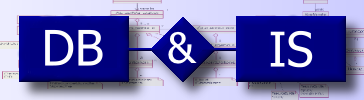
\includegraphics[height=\logoheight]{../latex_main/figures/DBIS_Kurzlogo.png}\qquad

\includegraphics[height=\logoheight]{../latex_main/figures/TNT_darkv4}\qquad

\includegraphics[height=\logoheight]{../latex_main/figures/L3S.jpg}	}
\date{Summer Term 2022; \hspace{0.5em} {
\includegraphics[height=1.5em]{../latex_main/figures/Cc-by-nc-sa_icon.svg.png}}; based on \href{https://ds100.org/fa21/}{[DS100]}
}


%%% Custom Packages
%----------------------------------------------------------------------
% Create dummy content
\usepackage{blindtext}

% Adds a frame with the current page layout. Just call \layout inside of a frame.
\usepackage{layout}


%%% Macros
%\renewcommand{\vec}[1]{\mathbf{#1}}
% \usepackage{bm}
%\let\vecb\bm

\title[Introduction]{DS: Inference for Modeling}
\subtitle{Inference}

\graphicspath{ {./figure/} }
%\institute{}


\begin{document}
	
	\maketitle
	\begin{frame}{Prediction vs. inference}
	    Prediction is the task of using our model to make predictions for the response of unseen data.\\
	    \bigskip
	    Inference is the task of using our model to draw conclusions about the underlying true relationship(s) between our features and response.\\
	    \bigskip
	    For example, suppose we are interested in studying the relationship between the value of a home and crime rates, a view of a river, school districts, size, income level of community, etc.
	    \begin{itemize}
	        \item Prediction: Given the attributes of some house, how much is it worth?
	        \begin{itemize}
	            \item Care more about making accurate predictions, don’t care so much about how.
	        \end{itemize}
	        \item Inference: How much extra will a house be worth if it has a view of the river?
	        \begin{itemize}
	            \item Care more about having model parameters that are interpretable and meaningful.
	        \end{itemize}
	    \end{itemize}
	\end{frame}
	
	
	\begin{frame}{What is statistical inference?}
	    \begin{itemize}
	        \item There is some fact we want to know about the population. This is called a population parameter.
	        \begin{itemize}
	            \item Formally, a parameter is a numerical function of a population. 
	        \end{itemize}
	        \item Accessing the entire population is infeasible (too expensive, too time-consuming), so we collect a random sample of the population.
	        \item We can compute a statistic of the random sample.
	        \begin{itemize}
	            \item A statistic is a numerical function of a sample.
	        \end{itemize}
	        \item However, that sample could have come out differently.
	        \begin{itemize}
	            \item For example: when we estimate the population mean given the sample mean, our guess is almost always going to be somewhat wrong.
	        \end{itemize}
	        \item Inference is all about drawing conclusions about population parameters, given only a random sample.
	    \end{itemize}
	\end{frame}
	
	
	\begin{frame}{Terminology}
	    Useful terminology:
	    \begin{itemize}
	        \item Parameter: Some function of a population (or “data generating process”).
	        \begin{itemize}
	            \item Denoted with    $\hat{\theta}$    .
	            \item Example: Population mean.
	        \end{itemize}
	        \item Estimator: Some function of a sample, whose goal is to estimate a population parameter.
	        \begin{itemize}
	            \item Denoted with $\hat{\theta}$    .
                \item Remember, random variables were functions of random samples.
                \item Hence, since we sample at random, estimators are random variables.
                \item Example: sample mean.
	        \end{itemize}
	        \item Sampling distribution: The distribution of estimator values, across all possible samples.
	        \begin{itemize}
	            \item This is unknown: we don’t have access to the population, so we don’t know what all possible samples look like.
	        \end{itemize}
	    \end{itemize}
	\end{frame}
	
	
	\begin{frame}{Bias and variance of an estimator}
	    Bias of an estimator: the difference between the estimator’s expected value and the true value of the parameter being estimated.
	    \begin{itemize}
	        \item Zero bias (unbiased): on average, our estimate is correct.
	        \item  Non-zero bias: on average, our estimate is consistently too large / too small.
	        \begin{equation*}
	            Bias[\hat{\theta}, \theta^*] = E[\hat{\theta}] - \theta
	        \end{equation*}
	    \end{itemize}
	    Variance of an estimator: the expected squared deviation of an estimator from its mean.
	    \begin{itemize}
	        \item The larger the variance of an estimator is, the more it varies from its own average.
	    \end{itemize}
	    \begin{equation*}
	            Var[\hat{\theta}] = E[(\hat{\theta} - E[\hat{\theta}])^2]
	        \end{equation*}
	\end{frame}
	
	
	\begin{frame}{Example: sample mean estimator}
	    What’s the variance of the sample mean estimator?
	    \begin{figure}
	        \centering
	        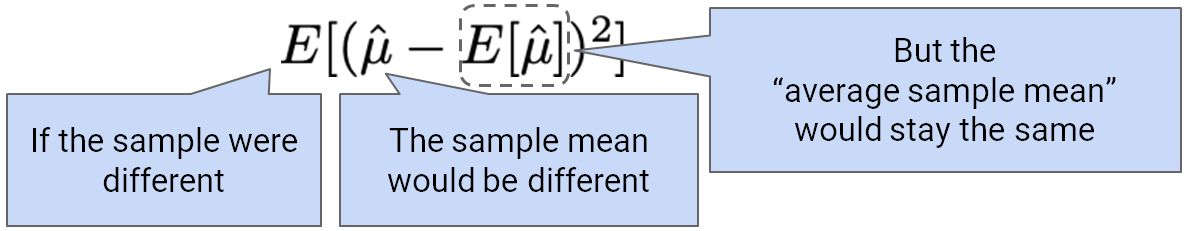
\includegraphics[scale=.45]{Bild1}
	    \end{figure}
	    \begin{itemize}
	        \item Note: We use hats to denote estimates.
	        \begin{itemize}
	            \item Think about how this relates to the “optimal thetas” that we also denoted with hats! 
	        \end{itemize}
	        \item Where’s the population mean,   $\hat{\mu^*}$    ?
	        \begin{itemize}
	            \item Variance isn’t about the population parameter, it’s about the estimator itself.
	        \end{itemize}
	        \item We can’t usually compute the expected value or variance of an estimator exactly!
	        \begin{itemize}
	            \item We’d need access to the true population.
	        \end{itemize}
	    \end{itemize}
	\end{frame}
	
	
	\begin{frame}{Example: estimating an estimator’s variance}
	    What’s the variance of the sample mean estimator?
	    \begin{figure}
	        \centering
	        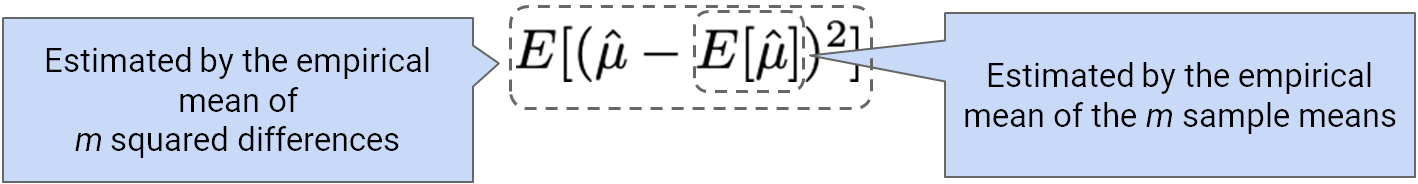
\includegraphics[scale=.4]{Bild2}
	    \end{figure}
	    Impractical approach that would work:
	    \begin{itemize}
	        \item Draw m different random samples of size n from the population.
	        \item For each sample, apply the estimator (i.e., compute the sample mean).
	        \item Estimate the variance of the estimator using the empirical variance of these estimates.
	    \end{itemize}
	\end{frame}
	
	\begin{frame}{Example: estimating an estimator’s variance}
	    Why is this so impractical?
	    \begin{figure}
	        \centering
	        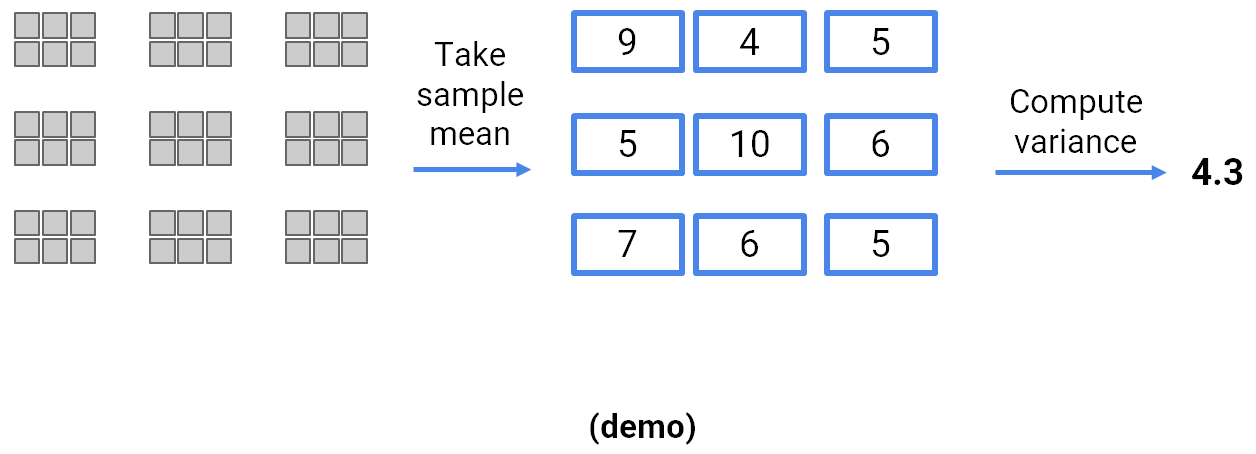
\includegraphics[scale=.4]{Bild3}
	    \end{figure}
	\end{frame}
\end{document}